\documentclass[../main.tex]{subfiles}

\begin{document}
\subsection*{Foreword}
This report was originally intended as a report for the course Introduction to Quantum Computing at the University of Twente. Both the report and the course are provided by ING employees. Initially, the report was meant to show maturity in quantum computing of the students attending the course. However, it became quickly interesting to upstream the report into a tutorial for, mostly colleagues, who would like to have a step-by-step introduction to quantum computing and to execute Monte Carlo simulations on such computers. The report is going to be a living document and will be updated from time to time as the field of Monte Carlo simulations on quantum computers advances and the author's experiences too. Lastly, the Monte Carlo simulations are applied in the domain of (quantitative) finance, thus, covering the financial problems too in the report. We hope that this report meets its requirements as a standalone document for the quantum computing enthusiasts in the financial world.

\section{Introduction}\label{sec: introduction}

% Computational Finance
Banks and other financial institutes employ vast computational resources for pricing and risk management of financial assets and derivatives. Without the computational resources evaluating complex mathematical models today's financial markets would be in grave danger and could not operate efficiently or at the scale it does nowadays. Examples of assets on financial markets are stocks, bonds and commodities. The assets are a base for more complex financial instruments called derivatives. A financial derivative, as it name suggests, derives its price from the future price or a price trajectory of at least one asset. As the nature of risky assets is stochastic, determining a fair price of a derivative (contract) is a challenge. A mathematical model that can be used for this pricing model is called the Black-Scholes-Merton model. In Section \ref{sec: bms} this model is discussed in more depth and its applications on derivatives is addressed.
\par

% Monte Carlo simulations
The Black-Scholes-Merton model is only solved analytically for very simple derivatives. For example, a simple derivative is a derivative whose payoff only relies on the future price at maturity time. A more complex derivative would be one where the payoff depends on the trajectory towards some future price at maturity time. Unfortunately, these complex derivatives have path-dependence embedded in the payoff function and combined with the stochastic nature of the underlying asset(s), it becomes infeasible (or perhaps impossible) to find an analytical solution for the pricing problem. Due to the stochastic nature of the underlying risky asset(s), it is wise to revert to a method where the expectation value of the future price (or the trajectory) is calculated by repeatedly and randomly sampling from a probabilistic distribution describing the underlying asset price (development). This method, called the Monte Carlo method, has long been explored in physics, chemistry, biology, finance, meteorology and many other domains where analytical solutions are infeasible and stochastic behaviors are observed. Random sampling from a distribution yield a higher accuracy (i.e., lower error) as the number of samples is growing. The downside of increasing the number of samples is the increased cost of computational power. A ten-fold improvement in accuracy suggests a hundred-fold longer runtime. Monte Carlo simulations can become rapidly intractable due to the scaling illustrated in the previous sentence. Thus, perhaps by changing the nature of deterministic processing units in computers to stochastic processing units, such as quantum processing units, a better scaling might be attained. Therefore, this report explores the opportunities and challenges of quantum computers regarding Monte Carlo simulations applied in the financial industry. For a more in-depth introduction on Monte Carlo simulations, please consult Section \ref{sec: mc}.
\par

% Exploring Quantum Computing and motivations
A quantum algorithm and computer capable of performing Monte Carlo simulations of financial derivatives (and the pricing problems) in a consistent and reliable way would be of utmost importance. This document discusses and shows which algorithms on quantum computers might be helpful in risk analytics and derivatives pricing.\par

% Exploring Quantum Computing and motivations
\subsection{Introduction to Quantum Computing} \label{sec: intro_qm}

% Qubit definition
\subsubsection*{Qubits, Measurement and Superposition}
Gated quantum computing is similar to classical computing with logical circuits. A logical circuits is composed of bits and gates. A bit is a binary digit carrying one of the following two values exclusively: $0$(\textit{false}) or $1$ (\textit{true}). A quantum bit, abbreviated as \emph{qubit}, is a quantum state with two base states $\ket{0}$ and $\ket{1}$ and does not exclude the presence of both states simultaneously (which is called the \emph{superposition} principle). How and how much a base state is contributing to the qubit is determined by the amplitude ($\alpha$, and $\beta$ in the equation below) of each base state. Upon measuring a quantum state, hence forcing it into a classical realm, the superposition principle collapses and only one single deterministic state must be acquired. The resulting state is retrieved by a stochastic process in which the probability distribution of the base states is characterized by the absolute value squared of amplitudes. As the sum of all probability coefficients of a probability distribution must be one, the sum of all absolute value squared of amplitudes must be one too. A qubit is then defined as the equation below following both an algebraic and a vector representation respectively:

\begin{equation}
    \ket{\psi} = \alpha \ket{0} + \beta \ket{1}, \, \,\text{with} \,\, (\alpha, \beta) \in \mathcal{C},
    \, \,\text{and} \, \, |\alpha|^2 + |\beta|^2 = 1   
    \label{eq: qubit_definition}
\end{equation}
 
\begin{equation}
    \ket{\psi} = \begin{bmatrix}\alpha \\ \beta \end{bmatrix}
    \label{eq: qubit_vector_representation}
\end{equation}

A visualization of a qubit is given according to a Bloch sphere as shown in Fig.\,\ref{fig: bloch_sphere}. A qubit may take any position on the whole surface of the Bloch sphere enforced by the constraint of having the sum of all probability coefficients to be one. The $z$-axis depicts the probability distribution of the base states of the qubit. Going higher or lower at the $z$-axis changes the probability distribution of the qubit. Hence, any operation acting on the qubit changing the qubit's position $z$-axis induces a \emph{state change}. The $x$-axis and $y$-axis depict the phase of a qubit, or more specifically, the relation between the two amplitudes of a qubit. On the $x$-axis the real values of the amplitudes are considered. If the qubit is pointing to the positive side of the $x$-axis, then the real values of the amplitudes have the same bias sign (either both $+$ or both $-$). If the qubit state vector is pointing to the negative side of the $x$-axis, the bias signs of the real values of the amplitudes differ, i.e., (one is $+$, other one is $-$). The $y$-axis regards the imaginary component of the amplitude from the second base state relatively to the imaginary component of the amplitude from the first base state. If the imaginary component is a shift of $+i$ or $-i$, the state vector would be pointing to the positive or negative side of the $y$-axis respectively. Any operation altering the values on the $x$ or $y$-axes is said to be inducing a \emph{phase change}.
\begin{figure}[H]
    \begin{center}
      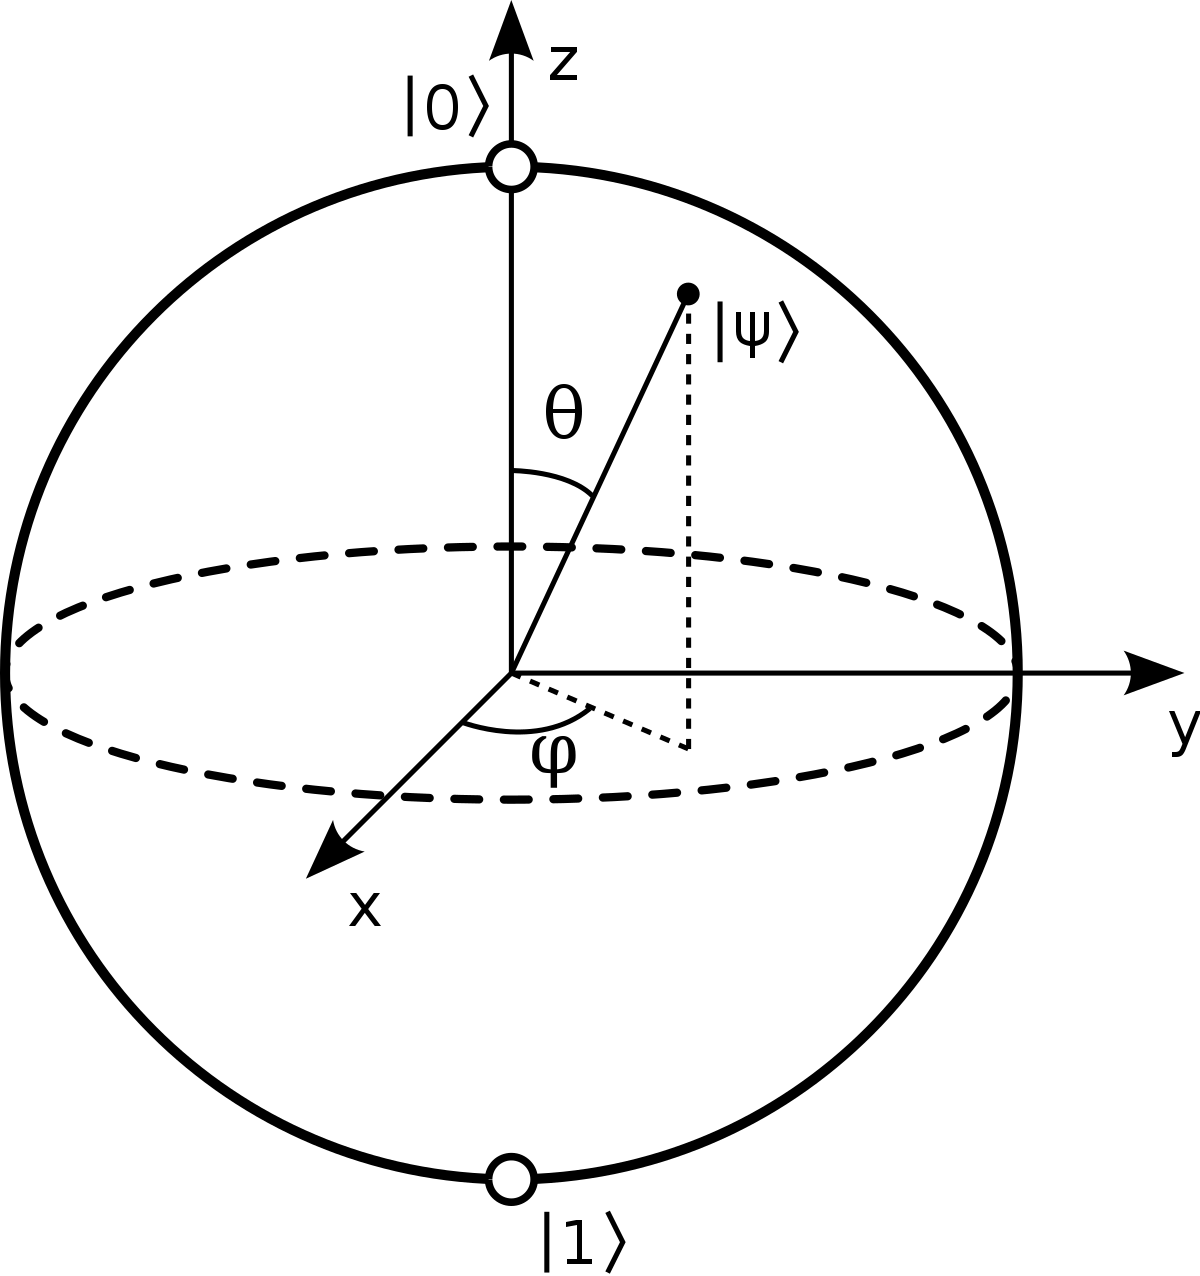
\includegraphics[width=0.5\linewidth]{../../images/bloch_sphere.png}
    \end{center}
    \caption{The Bloch sphere depicts the amplitudes of a qubit. The positive $x$-axis refers to: $\ket{+x} = \sqrt{1/2}(\ket{0} + \ket{1})$. The negative $x$-axis: $\ket{-x} = \sqrt{1/2}(\ket{0} - \ket{1})$. The positive $y$-axis refers to: $\ket{+y} = \sqrt{1/2}(\ket{0} + i \ket{1})$. The negative $y$-axis: $\ket{-y} = \sqrt{1/2}(\ket{0} - i \ket{1})$}
    \label{fig: bloch_sphere}
\end{figure} 
% \par

% Quantum Gates and X-gate
\subsubsection*{Quantum Gates}
Logical gates take in a Boolean input and return a Boolean output as followed from a Boolean function embedded in that gate. For example, a NOT-gate has a Boolean formula embedded in it that inverts the binary value of an input bit. To illustrate, an input bit with value 0 would become an output bit with value 1. A quantum gate follows the same principle. The quantum gate has an input quantum state (or an amplitude vector), follows a linear algebraic formula (or a matrix) and returns an output quantum state (again, an amplitude vector). One notable differenc between classical and quantum computing is the number of bits and qubits put in and returned. In classical computing the number of input and output bits may differ, for example, the AND-gate, would require two input bits and only returns a single output bit. In quantum computing a quantum gate performs on operation on (a set of) qubits and solely transforms the states of these qubits only. More technically, a quantum gate is a unitary matrix.  The unitary property, i.e., the complex conjugate transpose of a matrix multiplied by the original matrix is an identity matrix, ensures that the norm of the quantum state vector is preserved (and remains one). All unitary matrices are square too. The property of being square results in the fact that the number of qubits is preserved during the operation. An example of a quantum gate deployed on a single qubit is given below where the amplitudes of the base states are swapped:

\begin{gather}
    X = \begin{bmatrix} 
    0 & 1 \\
    1 & 0 \\
    \end{bmatrix} 
    \label{eq: gate_x}\\
    \text{Let } \ket{\psi} = \alpha \ket{0} + \beta \ket{1} = \begin{bmatrix}\alpha \\ \beta \end{bmatrix} \\
    X\ket{\psi} =  \begin{bmatrix} 
        0 & 1 \\
        1 & 0 \\
        \end{bmatrix} \begin{bmatrix}\alpha \\ \beta \end{bmatrix}  = \begin{bmatrix}\beta \\ \alpha \end{bmatrix} = \beta \ket{0} + \alpha \ket{1}
\end{gather}

% Quantum Circuit Representation
\subsubsection*{Quantum Circuits}
The above operation can be represented as a quantum circuit as seen below. The qubit is shown as a quantum register (and is often initialised with state $\ket{0}$). Gates are blocks put on a quantum register and perform an operation on the targetted qubit. The first gate denotes the X-gate operation as exemplified above. The second gate is a measurement gate. The measurement gate collapses the quantum state into a single deterministic base state according to the probability distribution derived from the amplitudes of the quantum state.

\begin{equation*}
    \begin{quantikz}[transparent]
        \lstick{\ket{\psi}} & \gate{X} & \meter{}
    \end{quantikz}
\end{equation*}

% Interference
\subsubsection*{Interference}
Qubits are technically quantum states, hence, are governed by a wave function as followed from/by Schrödinger's equation. The wave nature allows for \emph{interference} where amplitudes of a base state may constructively or destructively interfere. Below is an example of interference upon using an Hadamard gate on a generic qubit. The quantum circuit is also shown below.

\begin{gather*}
    H\ket{\psi} =  \sqrt{\frac{1}{2}}\begin{bmatrix} 1 & 1 \\ 1 & \text{-}1 \end{bmatrix} \begin{bmatrix}\alpha \\ \beta \end{bmatrix}  = \\ 
    \sqrt{\frac{1}{2}} \begin{bmatrix}\alpha + \beta \\ \alpha - \beta \end{bmatrix} = \\
    \sqrt{\frac{1}{2}}(\alpha + \beta) \ket{0} + \sqrt{\frac{1}{2}}(\alpha - \beta) \ket{1}
\label{eq: gate_h}
\end{gather*}

\begin{equation*}
    \begin{quantikz}[transparent]
        \lstick{\ket{\psi}} & \gate{H} & \meter{}
    \end{quantikz}
\end{equation*}

If $\alpha = \beta$, then the $\ket{1}$-state would be diminished completely. Even though the qubit started in a superposition of two base states, due to interference, the resulting qubit is now characterized by a single base state only. This does not mean the other base state is removed entirely, it is solely absent (until some other operation would redistribute the amplitudes such to acquire a non-zero amplitude on both base states).

% Multi-qubit systems
\subsubsection*{Multi-qubit systems}
A single qubit holds only two discrete base states representing two bits of information. Often, more bits of information is needed, thus more qubits are needed. With Boolean algebra and classical bits, multi-bit systems are $0$'s and $1$'s concatenaded horizontally from right to left. The right-most bit is the least significant bit, whereas the left-most bit is the most significant bit. For example, the integer number $13$ becomes the bit-string $1101$, where the left-most qubit is valued $2^{3} = 8$ and right-most qubit $2^0 = 1$. Qubits are represented in various ways, all meaning the same. 
\begin{gather*}
    \ket{1101} \\
    \ket{1,1,0,1} \\
    \ket{1} \ket{1} \ket{0} \ket{1} \\
    \ket{1} \otimes \ket{1} \otimes \ket{0} \otimes \ket{1} \\
\label{eq: multi_qubit_representation}
\end{gather*}
A four-qubit state holds $2^4 = 16$ bits of information. Therefore, the vector representing a four-qubit state has $16$ elements.

In a circuit, typically, but not always, the least significant bit is the uppermost qubit.  Now suppose a circuit is initialised with the state $\ket{1101}$ and some gates account for a final state $\ket{1000}$ (where an X-gate is put on the second and last qubit from the left).
\begin{equation*}
    \begin{quantikz}[transparent]
        \lstick{\ket{1}} & \gate{X} & \qw & \rstick{\ket{0}}  \\
        \lstick{\ket{0}} & \qw & \qw & \rstick{\ket{0}}  \\
        \lstick{\ket{1}} & \gate{X}& \qw & \rstick{\ket{0}}  \\
        \lstick{\ket{1}} & \qw & \qw & \rstick{\ket{1}} \\
    \end{quantikz}
\end{equation*}

Algebraically, these operations are represented as below by only picking the first and last qubit representation from above. Please note that the sequence of the Kronecker products ($\otimes$) is crucial. Here, $I$ is an identity matrix which preserves the same state (as multiplying any number by one with simple arithmetics).

\begin{gather*}
    (I \otimes X \otimes I \otimes X) \ket{1101} = \ket{1000}\\
    \\
    (I \otimes X \otimes I \otimes X) (\ket{1} \otimes \ket{1} \otimes \ket{0} \otimes \ket{1}) = \\
    I\ket{1} \otimes X\ket{1} \otimes I\ket{0} \otimes X\ket{1} = \\
    (\ket{1} \otimes \ket{0} \otimes \ket{0} \otimes \ket{0})
\label{eq: multi_quantum_circuit_representation}
\end{gather*}

% Kronecker Product
A Kronecker product is a tensor product between two tensors. Usually, the tensors used in quantum computing are often scalars, vectors and matrices. Below, two examples are given of Kronecker products to illustrate what it does. Let $\ket{\psi} = \alpha \ket{0} + \beta \ket{1}$ and $\ket{\phi} = \gamma \ket{0} + \delta \ket{1}$. The vector representation of these two states are respectively:

\begin{equation*}
    \ket{\psi} = \begin{bmatrix} \alpha \\ \beta \end{bmatrix}, \quad  \ket{\phi} = \begin{bmatrix} \gamma \\ \delta \end{bmatrix}
    \label{eq: kronecker_vector_definition}
\end{equation*}

Then the Kronecker product of the quantum states result in a composite quantum state:

\begin{gather*}
    \ket{\psi, \phi} = \ket{\psi} \otimes \ket{\phi} = \begin{bmatrix} \alpha \\ \beta \end{bmatrix} \otimes \begin{bmatrix} \gamma \\ \delta \end{bmatrix} \\
    = \begin{bmatrix} \alpha \begin{bmatrix} \gamma \\ \delta \end{bmatrix} \\ \beta \begin{bmatrix} \gamma \\ \delta \end{bmatrix} \end{bmatrix} \\
    = \begin{bmatrix} \alpha \gamma \\ \alpha \delta \\ \beta \gamma \\ \beta \delta \end{bmatrix}
    \label{eq: kronecker_vector}
\end{gather*}

A similar example is given for two $2 \times 2$-matrices called $U$ and $V$.

\begin{equation*}
    U = \begin{bmatrix} a & b \\ c & d  \end{bmatrix}, \quad  V = \begin{bmatrix} e & f \\ g & h  \end{bmatrix}
    \label{eq: kronecker_matrix_definition}
\end{equation*}

The Kronecker product of U and V is then:

\begin{gather*}
    U \otimes V = \begin{bmatrix} a & b \\ c & d  \end{bmatrix} \otimes \begin{bmatrix} e & f \\ g & h  \end{bmatrix} \\
    = \begin{bmatrix} a \begin{bmatrix} e & f \\ g & h  \end{bmatrix}
        & b \begin{bmatrix} e & f \\ g & h  \end{bmatrix}\\ 
        c \begin{bmatrix} e & f \\ g & h  \end{bmatrix}
        & d \begin{bmatrix} e & f \\ g & h  \end{bmatrix} \end{bmatrix} \\
        =  \begin{bmatrix} ae & af & be & bf \\ ag & ah & bg & bh \\ ce & cf & de & df \\ cg & ch & dg & dh  \end{bmatrix}
    \label{eq: kronecker_matrix}
\end{gather*}

A pattern that one sees above is that Kronecker products are about putting the rightmost tensor inside of the leftmost tensor in the equation multiplying the rightmost tensor by every scalar of the leftmost tensor.  

The inverse of a Kronecker product involves finding $A$ and $B$ from $C = A \otimes B$. There are no unique solutoins for this problem. However, one may consult the Pitsianis-Van Loan algorithm for the approximation of $A$ and $B$ by a minimisation function (if the two matrices are real valued). For the sake of illustration, consider the vector below:

\begin{equation*}
    x = \begin{bmatrix} 1 \\ 0 \\ 2 \\ 0  \end{bmatrix}
\end{equation*}

The goal is to find two vectors $u$ and $v$ such that $x = u \otimes v$. Just by trial and error one would find:

\begin{equation*}
    u = \begin{bmatrix} 1 \\ 2 \end{bmatrix}, \quad  v = \begin{bmatrix} 1 \\ 0 \end{bmatrix}
\end{equation*}

This means that a $4$-dimensional vector can be decomposed in two $2$-dimensional vectors. Regarding qubits, this would mean that a composed two-qubit system is decomposed in two independent qubits, as each independent qubit has only two elements in its vector representation.

% Entanglement
\subsubsection*{Entanglement}
It is possible to have a multi-qubit state in which it is not possible to invert the Kronecker product. Consider the following problem:

\begin{equation*}
    \ket{\psi} = \sqrt{\frac{1}{2}} \ket{00} + \sqrt{\frac{1}{2}} \ket{11} = \sqrt{\frac{1}{2}} \cdot \begin{bmatrix} 1 \\ 0 \\ 0 \\ 1 \end{bmatrix}, \quad  \text{ find } \ket{u} \text{ and } \ket{v} \text{ for which holds } \ket{\psi} = \ket{u} \otimes \ket{v}
\end{equation*}

It is not possible to find valid quantum states $\ket{u}$ and $\ket{v}$ for this problem, even though $\ket{\psi}$ is a valid two-qubit state. It is then said that the two qubits are strongly correlated, or entangled, meaning that that $\ket{\psi}$ acts like a single particle composed of two strongly correlated qubits. Suppose $\ket{\psi} = \sqrt{\frac{1}{2}} \ket{00} + \sqrt{\frac{1}{2}} \ket{11}$ to be measured and the leftmost qubit is measured. There is a probability of $\dfrac{1}{2}$ that the leftmost qubit will collapse in a $0$-state or in a $1$-state. However, it would collapse into a $0$-state, then the remaining qubit is also going to be in a $0$-state as it is the only option left. With that, the superposition of the second qubit immediately collapses when the first qubit is measured. One bit of measurement hence gives two bits of information, one can say.

Entanglement is useful in many occassions in quantum computing. Suppose an initial two state system to be $\ket{x}\ket{0}$ and that there is a quantum gate that embeds a function $f(x)$ that provides $\ket{x}\ket{f(x)}$. By entanglement, any input $x$ is connected to its corresponding output $f(x)$. If the input-register is a superposition of many states, i.e., many inputs, then the output-register will host a superposition of many outputs at the same time. It is therefore not a surprise that including superposition and entanglement into a quantum circuit leverages speedups. With interference included in the post-processing of the superposed and entangled circuit, algorithms can be designed that might give speedups to classical counterparts.

% Parameterized Quantum Circuits
\subsubsection*{Parameterized Quantum Circuits}
Gates are unitary matrices, meaning, that the complex conjugate transpose of a square matrix times the original matrix should be equal to an identity matrix (with the same dimensions as the original matrix). This is illustrated by the equation below where $U$ is any unitary matrix.

\begin{equation}
    U^\dagger U = \mathcal{I}
\end{equation}

Earlier, the $X$-gate and the $H$-gate were presented. The elements of these two matrices are fixed scalars. It is possible to construct unitary matrices that have variable scalars. For example, the $U_3$-gate has three parameters that may traverse the whole Bloch sphere as depicted in Fig.\,\ref{fig: bloch_sphere}. 

\begin{equation}
    U_3(\theta, \phi, \lambda) =
    \begin{pmatrix}
        \cos(\theta)          & -e^{i\lambda}\sin(\theta) \\
        e^{i\phi}\sin(\theta) & e^{i(\phi+\lambda)}\cos(\theta)  
    \end{pmatrix}
\label{eq: u3-gate}
\end{equation}

Taking $\theta = \frac{\pi}{2}$, $\lambda = \pi$ and $\phi = 0$ would give the same matrix as the $X$-gate (see Eq.\,\ref{eq: gate_x}). The parameters are defined before the execution of a quantum circuit. Such gates are called \emph{parameterized} and make hybrid classical-quantum computing possible. It is also advantageous for users to specify a certain quantum states as desired without putting much effort in collecting a multitude of non-parameterized gates approximating the desired state.  

% Variational Quantum Computing
Parameterized quantum circuits open the door to include classical computational methods in quantum circuits. The idea is as follows:
\begin{enumerate}
    \item Build a parameterized quantum circuit containing some (elements) of an objective function (or a loss function).
    \item Initialize a vector of parameters to be put in the circuit. The elements can be randomized or user-defined.
    \item Run the circuit and measure the outcomes (optionally, measure the outcomes according to some observable).
    \item Use the outcome of the circuit as an input for a loss function.
    \item Use a classical optimizer to readjust the parameters and re-run the circuit.
    \item Repeat steps (3-5) until the loss function has been optimized according to a given tolerance level.
\end{enumerate}

An illustration of the steps above is given below:

\begin{figure}[H]
    \begin{center}
      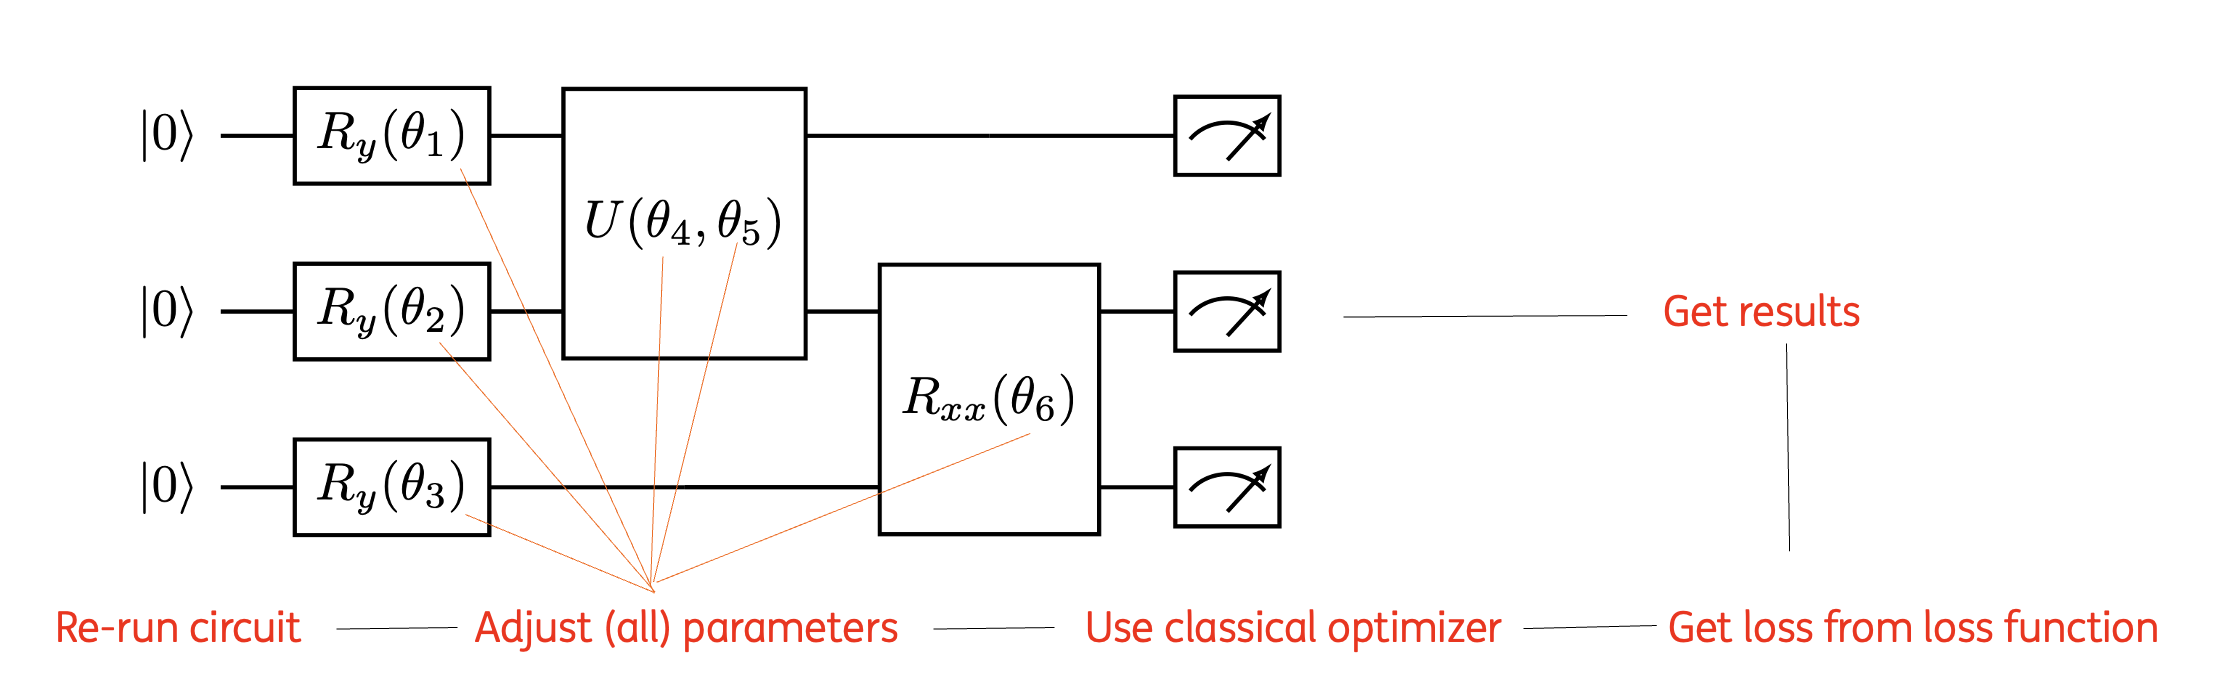
\includegraphics[width=1\linewidth]{../../images/variational_circuit_example.png}
    \end{center}
    \caption{An illustration of a variational quantum circuit. A quantum circuit acts as an outer-loop for optimizations. This circuit has six parameters over five different gates. The circuit is run, results are retrieved and evaluated according to a loss function. Subsequently, a classical optimizer is used to find or try new parameters that may optimize the loss function.}
    \label{fig: variational_circuit_example}
  \end{figure}

Variational quantum circuits are very handy for many applications. For one, discrete and continuous functions can be optimized. Secondly, it can be interpreted as a neural network with a classical optimizer, rendering quantum neural networks possible. Thirdly, extending the idea of the previous point, such circuits can be used to generate quantum data from classical data. 

\biblio
\end{document}
